\documentclass[11pt, a4paper]{report} % add draft if needed

\usepackage[english]{babel}
\usepackage[T1]{fontenc}
\usepackage[utf8]{inputenc}
\usepackage{mathtools}
\usepackage{amsfonts}
\usepackage{listings}
\usepackage[a4paper]{geometry}
\usepackage[parfill]{parskip}
\usepackage{hyperref}
\usepackage{lipsum}
\usepackage[toc,page]{appendix}
\usepackage{lastpage}
\usepackage{fancyhdr}
\usepackage[explicit]{titlesec}
\usepackage{color}
\usepackage{amsthm}
\usepackage{todo}
\usepackage{tikz}
\usepackage{subcaption}
\usepackage{caption}
\usepackage{chemfig}
\usepackage{cleveref}
\usepackage{minted}

\providecommand{\tightlist}{%
  \setlength{\itemsep}{0pt}\setlength{\parskip}{0pt}}

\setminted{linenos,frame=lines,framesep=2mm}
\setminted[text]{linenos=false}


%tikz extras
\usetikzlibrary{arrows, shapes, snakes, automata, backgrounds, positioning}

\tikzset{
    triple/.style args={[#1] in [#2] in [#3]}{
        #1,preaction={preaction={draw,#3},draw,#2}
    }
}

%chemo macros
\newcommand{\cheminl}[1]{$\mathrm{#1}$}

% math envirs
\newtheorem{defin}{Definition}
\newtheorem{theo}{Theorem}

% Chapter title formatting
\definecolor{gray75}{gray}{0.75}
\newcommand{\hsp}{\hspace{20pt}}

\titleformat{\chapter}[display]{}{
}{-85pt}{\Huge\bfseries\centering\textcolor{gray75}{|}\hsp#1\hsp\textcolor{gray75}{|}\\\hspace{10pt}}

% Header and footer
\fancypagestyle{plain}{% plain style is used on chapter pages
  \fancyhf{}%
  \fancyfoot[C]{\thepage}% Page \thepage\ of \pageref*{LastPage}
  \renewcommand{\headrulewidth}{0pt}% Line at the header invisible
  %\renewcommand{\footrulewidth}{0.4pt}% Line at the footer visible
}

\pagestyle{fancy}
\fancypagestyle{MyStyle}{
    \fancyhf{}
    \fancyhead[L]{ \leftmark }
    \fancyhead[R]{ \today }
    \fancyfoot[C]{ \thepage } % chktex 2
    \renewcommand{\chaptermark}[1]{\markboth{\textsl{##1}}{}}
    \renewcommand{\headrulewidth}{0pt}
}

\newcommand{\blankpage}{
  \newpage
  \thispagestyle{empty}
  \mbox{}
  \newpage
}

% \definecolor{mygreen}{rgb}{0,0.6,0}
% \definecolor{mygray}{rgb}{0.5,0.5,0.5}
% \definecolor{mymauve}{rgb}{0.58,0,0.82}

% \lstset{ %
%   backgroundcolor=\color{white},   % choose the background color; you must add \usepackage{color} or \usepackage{xcolor}; should come as last argument
%   basicstyle=\footnotesize,        % the size of the fonts that are used for the code
%   breakatwhitespace=false,         % sets if automatic breaks should only happen at whitespace
%   breaklines=true,                 % sets automatic line breaking
%   captionpos=b,                    % sets the caption-position to bottom
%   commentstyle=\color{mygreen},    % comment style
%   deletekeywords={...},            % if you want to delete keywords from the given language
%   escapeinside={\%*}{*)},          % if you want to add LaTeX within your code
%   extendedchars=true,              % lets you use non-ASCII characters; for 8-bits encodings only, does not work with UTF-8
%   frame=single,                       % adds a frame around the code
%   keepspaces=true,                 % keeps spaces in text, useful for keeping indentation of code (possibly needs columns=flexible)
%   keywordstyle=\color{blue},       % keyword style
%   language=Octave,                 % the language of the code
%   morekeywords={*,...},           % if you want to add more keywords to the set
%   numbers=left,                    % where to put the line-numbers; possible values are (none, left, right)
%   numbersep=5pt,                   % how far the line-numbers are from the code
%   numberstyle=\tiny\color{mygray}, % the style that is used for the line-numbers
%   rulecolor=\color{black},         % if not set, the frame-color may be changed on line-breaks within not-black text (e.g. comments (green here))
%   showspaces=false,                % show spaces everywhere adding particular underscores; it overrides 'showstringspaces'
%   showstringspaces=false,          % underline spaces within strings only
%   showtabs=false,                  % show tabs within strings adding particular underscores
%   stepnumber=2,                    % the step between two line-numbers. If it's 1, each line will be numbered
%   stringstyle=\color{mymauve},     % string literal style
%   tabsize=2,                       % sets default tabsize to 2 spaces
%   title=\lstname                   % show the filename of files included with \lstinputlisting; also try caption instead of title
% }

\title{Building a Package Manager for Jolie}
\author{Dan Sebastian Thrane}

\begin{document}
\begin{titlepage}

\newcommand{\HRule}{\rule{\linewidth}{0.5mm}} % Defines a new command for the horizontal lines, change thickness here

%\ % Center everything on the page
\flushright %centering
%----------------------------------------------------------------------------------------
%   LOGO SECTION
%----------------------------------------------------------------------------------------
%\begin{minipage}{0.9\textwidth}
%\centering
%\hspace*{2cm}
%

\includegraphics[scale=0.35,bb=0 0 250 0]{pictures/SDU_logo.eps}\\[1cm] % Include a department/university logo - this will require the graphicx package

%----------------------------------------------------------------------------------------
%   HEADING SECTIONS
%----------------------------------------------------------------------------------------

\textsc{\LARGE University of Southern Denmark}\\%[0.3cm] % Name of your university/college
\textsc{\normalsize Department of Mathematics and Computer Science,\\ IMADA}\\[2.6cm]
 % Major heading such as course name
 % Minor heading such as course title

%----------------------------------------------------------------------------------------
%   TITLE SECTION
%----------------------------------------------------------------------------------------
\textsc{\Large Master Thesis}\\[0.5cm]
\hfill \\%[0.10cm]
{ \Huge \bfseries Building a Package Manager for Jolie }\\[0.4cm] % Title of your document
\hfill \\[2.8cm]

%----------------------------------------------------------------------------------------
%   AUTHOR SECTION
%----------------------------------------------------------------------------------------
\large
\emph{Author:}\\
Dan Sebastian \textsc{Thrane} % Your name
\\[0.8cm]
%~
\large
\emph{Supervisor:} \\
Fabrizio \textsc{Montesi} % Supervisor's Name


\vfill
% If you don't want a supervisor, uncomment the two lines below and remove the section above
%\Large \emph{Author:}\\
%John \textsc{Smith}\\[3cm] % Your name

%----------------------------------------------------------------------------------------
%   DATE SECTION
%----------------------------------------------------------------------------------------

{\large \today}%\\[2cm] % Date, change the \today to a set date if you want to be precise
%\end{minipage}

\end{titlepage}



\tableofcontents

\blankpage

\pagestyle{MyStyle}

\chapter{Introduction}
\section{Introduction}

TODO This is just an introduction to the CLI. Re-write to match the package
manager overall

The command line application serves as the user interface to JPM. The
application is, perhaps not unsurprisingly, named \mintinline{text}{jpm}. The
tool will be used in several examples.

The command line application is responsible for displaying a more user friendly
interface to inner workings of JPM. The tool will perform almost not work by
itself, but will instead delegate this to the back end (See Section TODO).

When first running the tool, the user will be welcomed with the following
message:

\begin{minted}{text}
JPM - The Jolie Package Manager
Version 1.0.0

Usage: jpm <COMMAND> <COMMAND-ARGUMENTS>

Command specific help: jpm help <COMMAND>

Available commands:
-------------------
init           Initializes a repository
search         Searches repositories for a package
install        Install dependencies
publish        Publish this package
start          Start this package.

[ Remaining commands removed from snippet ]
\end{minted}

As clearly visible form this snippet, for the tool to do any work we must first
give it something to do via a command. The commands that JPM understands almost
directly mirror the functionality provided by the back end. To use JPM to
create a new package, the user must simply use the \mintinline{text}{init}
command. This will display a prompt, guiding the user through the mandatory
field, and automatically create a package with the required structure. This
is shown in Listing \ref{lst:jpm_init}.

\begin{listing}[H]
\begin{minted}{text}
$ jpm init
Package name
------------
> my-package

Package description
-------------------
> This is my package

Author: [Format: name <email> (homepage)]
-----------------------------------------
> Dan Sebastian Thrane <dathr12@student.sdu.dk> (github.com/DanThrane)

Private package? [Y/n]
----------------------
> n

$ cat my-package/package.json | json name
my-package
\end{minted}

\caption{The \mintinline{text}{jpm} tool provides a user interface for common
    tasks. In this example, creating a new package.}

\label{lst:jpm_init}

\end{listing}





\chapter{Background}
Background goes here.

\section{Microservices}

\begin{itemize}
\item General stuff about microservices, actually introduce the thing
\end{itemize}

\section{Package Managers}

In this thesis we will work solely with application-level package managers.
As mentioned in the introduction, application-level package managers deal with
application-level packages. These packages are typically software components.

The work on the Jolie Package Manager (JPM), which this thesis presents, is
hugely inspired by the following works:

\begin{enumerate}
    \item \textbf{NPM:} The package manager for Node.js\autocite{NPMC}.
    \item \textbf{Yarn:} An alternative package manager for 
    Node.js\autocite{YARNC}.
    \item \textbf{Cargo:} Build tool for the Rust language\autocite{CARB}.
    \item \textbf{Gradle:} Build tool, typically used for JVM languages
    (e.g. Java)\autocite{GRAB}.
\end{enumerate}

In the remainder of this section we will cover the most common traits from
these works.

The primary role of a package manager, as the name would suggest, is to manage
software packages. A package manager usually describes software packages
through a special file, in this thesis we will refer to this file as the
package manifest. NPM and Yarn both use a file called \txtl{package.json},
Cargo uses a \txtl{Cargo.toml}, Gradle using a \txtl{build.gradle}.
Common for all of these are, that they typically describe the package itself,
and the dependencies of this package.

Listing \ref{lst:cargo_example} shows an example for Cargo, and shows a similar
manifest for NPM is shown in Listing \ref{lst:npm_example}. Common to both of
these examples, is that their descriptions use a few attributes for describing
the package itself. Additionally they have a section describing the
dependencies, i.e., the packages that should be ``managed''. Most importantly of
the attributes describing the package are the ``name'' and ``version'', which
can uniquely refer to a specific version of the package.

\begin{listing}[H]
\begin{minted}{ini}
[package]
name = "my-cargo-crate"
version = "1.2.3"
authors = ["Dan Sebastian Thrane <dathr12@student.sdu.dk>"]

[dependencies]
log = "0.3.8"
left-pad = "1.0.1"
\end{minted}
\caption{A simple manifest for a Cargo package (a ``Crate'')}
\label{lst:cargo_example}
\end{listing}


\begin{listing}[H]
\begin{minted}{json}
{
  "name": "my-npm-package",
  "version": "1.0.0",
  "description": "This is a NPM package",
  "main": "index.js",
  "scripts": {
    "test": "echo \"Error: no test specified\" && exit 1"
  },
  "author": "Dan Sebastian Thrane <dathr12@student.sdu.dk>",
  "license": "ISC",
  "dependencies": {
    "left-pad": "^1.1.3"
  }
}
\end{minted}
\caption{A simple manifest for a NPM package}
\label{lst:npm_example}
\end{listing}

Most package managing tools come with CLI (Command-Line Interface) tools, which
help the user perform various tasks. For example, both of the manifest examples
(Listing \ref{lst:cargo_example}, and \ref{lst:npm_example}) could be generated
via their respective tools as shown in Listing \ref{lst:tools_example}.

\begin{listing}[H]
\begin{minted}{text}
dan@host:/ # cargo new my-cargo-package
    Created library `my-cargo-package` project

dan@host:/ # npm init
This utility will walk you through creating a package.json file.
It only covers the most common items and tries to guess sensible defaults.

( ... Cut for brevity ... )
\end{minted}
\caption{Package managers typically ship CLI tools which help with common
    tasks}
\label{lst:tools_example}
\end{listing}

Similarly these tools can be used to download and install their dependencies,
for Cargo \txtl{cargo build}, for NPM \txtl{npm install}. The
packages, that these dependencies resolve to, can be stored in
various places. A common approach, which we see both NPM, Yarn, and Cargo, is
to use a default centralized registry. Gradle uses a similar approach but
doesn't have a single default registry (which they refer to as repositories).
The registries will act as a database of packages, which the tools will use
to download, and install packages. Registries typically also have some type of
user management. Such a feature becomes relevant when controlling who is
allowed to publish updates for a package.

The reader may have observed already, that we have been referring to both Cargo
and Gradle as package managers, even though they were listed as build tools.
The build tool description is pulled directly from their own descriptions.
However, the border between package managers and build tools are typically
blurry. Especially because many modern tools include dependency management as a
core part of their features. Even tools, like NPM, which advertise themselves
still build provide ``build tool''-like features, such as running tests and
starting the application. In this thesis, we will simply refer to our own tool,
the Jolie Package Manager, as a package manager. This is done, since
it is its primary responsibility, and technically there is nothing to
build in Jolie, due to its dynamic nature.

% Status: draft

\section{Introduction to Jolie}

Jolie is a service-oriented programming language, and is build to support a
microservice natively. In this section we will cover what kind of language
Jolie is, and how it is currently used.

Jolie has a C-inspired syntax, and is dynamically typed. Its interpreter is
written in Java.

The language has no native functions or methods, but instead works in
processes. A process has no arguments, and does not contain any stack (in the
case of recursive calls). There are two pre-defined processes, which will
always be called by the interpreter, these are called \verb!init! and
\verb!main!.

\begin{listing}[H]
\begin{minted}{jolie}
include "console.iol"

define PrintOutput {
    println@Console(output)() // Prints 'OK'
}

init { a = 1 }

main {
    b = 2;
    c = a + b; // c = 3
    if (c == 3) {
        output = "OK"
    } else {
        output = "Bad"
    };
    PrintOutput // Calls the defined process 'PrintOutput'
}
\end{minted}
\caption{A very simple Jolie program}
\label{lst:simple_jolie}
\end{listing}

Listing \ref{lst:simple_jolie} shows a very simple programming language, in
what looks like what you might expect from a dynamic language with C-inspired
syntax. However a few things may also strike you as odd.

First of all there are typos on lines 12, 14 or 16, the semicolon is not needed
here, in fact it would be a syntax error. The reason for this is that the
semicolon isn't used strictly for parsing purposes, but it instead for having
multiple statements in a process. The "semicolon" statement, also called a
sequence statement, has a syntax of \verb!A ; B!, which should be read as:
first perform statement \verb!A!, then perform \verb!B!. The sequence
statement requires both of the operands to be present, hence the syntax error.
Another similar statement is the parallel statement, which has a syntax of
\verb!A | B!, which reads as: do \verb!A! and \verb!B! in parallel. Using
these operators together allows the programmer to easily create a fork-join
workflow. This is typically used in microservices when we want to collect
data in parallel, and continue once all of the data has been retrieved.

Secondly has slightly different rules for scoping. In Jolie everything not
defined in the global scope goes into the same scope. This also persists
through calls to defines. This is the reason that \verb!PrintOutput! can use
the output variable.

Several execution modes exists. The default execution mode, which was used in
Listing \ref{lst:simple_jolie} is \verb!single!. This means that the
\verb!main!  process is run just a single time. Two more modes exists, those
being \verb!concurrent! and \verb!sequential!. TODO Some more stuff

Ports are the primitive that Jolie uses for communication, two types of ports
exists: input and output. Ports describe a running service, where it is located
(\verb!Location!), and how to speak to it (\verb!Protocol!), and finally which
operations it supports (\verb!Interfaces!). In Listing \ref{lst:simple_port} we
see a simple output port which contacts \verb!example.com! on port 42000, using
\verb!http!. Note that it is only the ports that deal with the protocol,
everything inside of the code is completely agnostic with respect to the
protocol being used for communication. As a result it is easy to change a
service from communicating using one protocol to another.

\begin{listing}[H]
\begin{minted}{jolie}
outputPort Example {
    Location: "socket://example.com:42000"
    Protocol: http
    Interfaces: IExample
}
\end{minted}
\caption{A simple output port which contacts the Google website}
\label{lst:simple_port}
\end{listing}

The interface which the port uses is called \verb!IExample!, a full definition
of it can be seen in Listing \ref{lst:simple_interface}. Two types of
operations exists in Jolie, namely \verb!RequestResponse! and \verb!OneWay!.
The difference being fairly self-explanatory, the first receives a request and
returns a response, the other simply receives a request, and produces no
response.

\begin{listing}[H]
\begin{minted}{jolie}
interface IExample {
    RequestResponse:
        anOperation(RequestType)(ResponseType)

    OneWay:
        hello(HelloType)
}
\end{minted}
\caption{An interface in Jolie defines which operations a port exposes}
\label{lst:simple_interface}
\end{listing}

Whenever the Jolie interpreter invokes an operation on an output port, or
receives a request on an input port, the types will be checked. This check
ensures that we don't send out incorrect requests, and ensures that we do not
attempt to process an incorrect request. Listing \ref{lst:simple_types} show
the request and response type of \verb!anOperation!.

\begin{listing}[H]
\begin{minted}{jolie}
type RequestType: void {
    .a: int
    .b: string
    .c: bool
    .d: double
    .e: any // any primitive type
}

type ResponseType: int {
    .aFixedArray[1, 3]: string
    .aNonFixedArray[0, *]: string
    .fieldWithChildren: void {
        .a: void {
            .b: int
        }
    }
}
\end{minted}
\caption{Jolie types are tree-like structures}
\label{lst:simple_types}
\end{listing}

In Jolie types are tree-like structures, very similar to how, for example, XML
would be represented. Importantly the root may also contain a value, this is
different from how most other programming languages work. This also means that
certain encodings may have problems with this. JSON a popular format for
serialization does not support root values, as a result Jolie will encode the
root value under a special key to work around this fact.

TODO Actually use this illustration for something, should probably work with
the actual example provided.

\begin{listing}[H]
\begin{minted}{text}
                         +----------+
                         |          |
                         +----------+
                              /\
                             /  \
                            /    \
                           /      \
                    +------+      +-------+
                    |      |      |       |
                    +------+      +-------+
                     /  |  \
                    /   |   \
                   /    |    \
                  /     |     \
          +-------+ +------+ +--------+
          |       | |      | |        |
          +-------+ +------+ +--------+
\end{minted}
\end{listing}

Jolie natively supports a variety of techniques for composition of services.
The most important (for this work), which we will cover here are
\textbf{aggregation} and \textbf{embedding}.

Embedding allows for a larger service to run smaller services as inner
components. These services communicate with each other using more efficient
local communication. These embedded services can be other Jolie services, but
may also be services written in, for example, Java or even JavaScript.
Communicating with these services is done exactly the same way as with any
other service, it is entirely transparent to the application code where the
service is located. TODO Can probably say a few more words about this subject.
Might be easier to add this later when we know what we actually need.

Aggregation is a generalisation of proxies and load balancers. An illustration
of this concept can be seen in Figure \ref{fig:aggregation}. Aggregation is
useful for creating a wide variety of proxy like architectural patterns. The
aggregation feature is often used along side the courier and interface extender
features. Couriers allows the developer to insert code in-between the receiving
the request and forwarding it. These features for example allow you to add
authentication to a service which otherwise doesn't have it. This is done
entirely without having to touch the original service.

\begin{figure}[H]
    \centering
    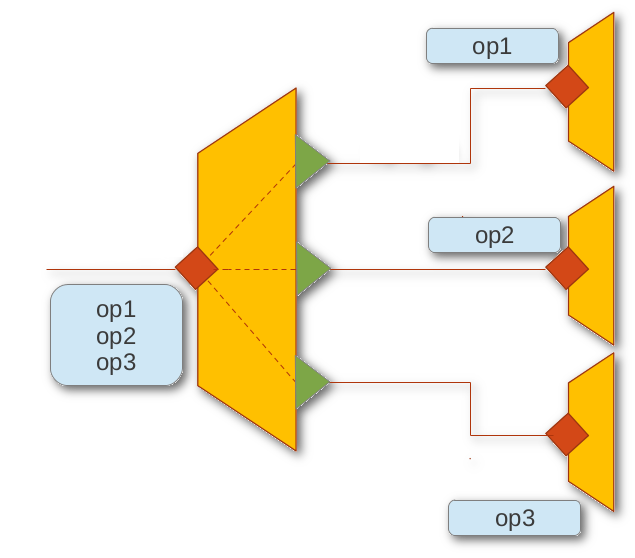
\includegraphics[width=0.6\textwidth]{pictures/aggregation.png}
    \caption{Aggregation is a generalisation of proxies and load balancers}
    \label{fig:aggregation}
\end{figure}


\section{The Jolie Engine and Interpreter}

In this section, the internals of the Jolie engine will be introduced. This
should give the reader the necessary knowledge to understand the changes made
to support a module and package system for Jolie.

At the core of the Jolie engine is the interpreter. Each interpreter is
responsible for parsing and executing a Jolie program. A single engine may run
several instances of the interpreter, this is most commonly the case when
embedding several other Jolie services.

A simplified view of the Jolie interpreter's pipeline can be seen in Figure
\ref{fig:jolie_pipeline}.

\begin{figure}[H]
\centering

\includegraphics[width=0.8\textwidth]{background/pipeline.eps}
\caption{A simplified view of the Jolie interpreter pipeline}
\label{fig:jolie_pipeline}
\end{figure}

The first phase of the interpreter is parsing the intent. In this phase the
interpreter will determine its purpose and, if any, modifiers to its ordinary
behavior.

The Jolie engine can be invoked from the command-line, the command-line is the
source of the intent which starts the first interpreter. The syntax for the
command line is (roughly) as follows: \txtl{jolie [commands and options]
    <program> [program arguments]}.

Options change the overall behavior of the engine, all interpreter instances
share these. These change the behavior of the interpreter.

Commands and program arguments, only belong to the interpreter that they were
originally passed. These determine what the interpreter will do.

The intent parsing phase is responsible for locating and retrieving the program
used.

A URI matching the input program is given to the program parser, the second
phase. The parser is responsible for creating the Abstract Syntax Tree (AST)
    which represents the input program. The parser will produce only a single
    root node, namely the \txtl{Program} node. Includes are thus implemented by
    essentially inserting the contents of the include target. A quirk for Jolie
    includes, is that relative file includes are not resolved relative to the
    current file, but rather to the current working directory (i.e. where the
            engine was started).

The third phase traverses the AST to make sure that it is semantically valid.
This weeds out programs that are syntactically correct, but not semantically
valid. The checks performed in this phase are somewhat limited, given the
dynamic nature of the language.

Given a semantically valid AST the interpreter is ready to build the
interpretation tree. The interpretation tree contains new nodes, which are
runnable.

Once the interpretation tree is built, we're ready to execute the actual code
(which lives in the interpretation tree). The \txtl{CommCore} component is
responsible for all communication, we'll discuss this briefly when relevant.
Following its initialization, the user code of Jolie will start executing. The
\joliel{init} procedure is executed first followed by the \joliel{main}
procedure.



\chapter{Jolie Modules}
\section{Summarizing the Problem}

The goal of this thesis is to promote, and facilitate better code reuse in
Jolie. In Section \ref{sec:complete} we showed how a typical Jolie service
would be written, and summarized a number of patterns we have observed.


\section{Modules: Design and Implementation}

A module in Jolie is defined as a project root directory, and optionally an
entry-point. Modules are uniquely identified by a name.

The Jolie engine needs to know about these modules. The engine is informed
about these modules from the intent, passed as options, which starts the
engine. This information is collected in the ``intent parsing'' phase, and is
made available to any later phase that might need it.  Since the intent is
passed as an option, all interpreter instances inside the engine will know
about each module.  As a result any embedded service will also be aware of the
same modules.

As an example, we may inform the engine about a module called ``foo'', which
has its source code placed in \verb!/packages/foo!  with an entry-point in
\verb!/packages/foo/main.ol! we would write: \mintinline{text}{--mod
foo,/packages/foo,main.ol}. This implementation technique is very close to
how, for example, you would add a JAR file to the classpath of a Java program.
% TODO Very informal argument

The result of this decision is that quite a lot of additional options may need
to be passed to the engine. However this choice was purposely chosen, it is
left for another tool to make this job easier. In this case a package manager
is expected to take the heavy lifting, and figure out which modules exists.
This allows for more freedom in how these tools are implemented, and another
implementation strategy, than the one provided in the package manager, could be
created without any changes to the language infrastructure. See Section TODO
about how the package manager passes this information to the engine.

To allow for better organization, a new type of include has been added to the
language. These include allows the developer to include from a particular
package. The syntax of this include is shown in Listing \ref{lst:mod_include}.
When a package include is used, the search path will be altered, such that the
project root is changed to that of the package (as opposed to where the engine
was started). Any file included from within this package should perform its
includes relative to its own root, rather than the project root.

TODO Example

The new include syntax, along with native support for modules, allows for the
code to properly organized. With this a module may be placed inside of its own
directory, without any of the code having to be changed.

\begin{listing}[H]
\begin{minted}{jolie}
include "<file>" from "<module>"
\end{minted}
\caption{Extension to the include statement, made for module imports}
\label{lst:mod_include}
\end{listing}

\subsection{Include Algorithm for Jolie}

TODO To this date I still don't understand how the include algorithm works. Ask
Fabrizio about this.

\subsection{Module Include Algorithm}

TODO Module includes modify the search path. This also means the injection of
the include directory, which is used as a convention. This helps maintain
expected behaviour.

TODO In order to implement the root switching we use a stack.

\section{Configuration}

% TODO Define configuration and which constructs we want to be configurable

\subsection{Motivation}

From observation 2 we saw that most configuration was done via the inclusion of
source code. This source code would expose constants (read: literal values
\emph{and} identifiers). The included source code, however, can do anything
that Jolie source normally can, and isn't limited to just the desired
configuration. As a result, a service developer cannot be certain that the
configurator (entity who provides configuration) doesn't start messing with
other details of the program. Deploying defensive
programming\footnote{Defensive programming techniques are usually employed for
systems that require high availability, or where safety and security is
required.} techniques against this becomes significantly more problematic,
since no guarantees about the configuration source file can really be made.

Distributing re-useable packages is also problematic with this approach.
Several features of package management namely requires that the package remains
read-only. Features that typically need this aspect could be updating, without
this we would need source-code merges, or integrity checks of packages.

We also saw that a lot of issues, that should have been purely deployment,
became a code problem.

This gives us plenty of reason to explore the need for a configuration format.
Most other systems would most likely go for a system defined in user code, as
opposed to natively in the language. An example of such framework, could be
Vert.x, it is a tool-kit for building reactive applications on the JVM.
Examples of such ``reactive applications'' are microservices. The configuration
workflow is shown in Figure \ref{fig:normal_conf}. The system will retrieve,
and read external configuration files, directed by the user code and apply the
configuration as needed.

% Most other systems can do this at run time
% For example Vert.x does this by reading external configuration files
% Once configuration is done, we can start up the server

\begin{listing}[H]
\begin{minted}{text}
+------------------+     +-------------------+     +--------------------+
| executable start | --> | retrieve conf     | --> | read conf files    |
+------------------+     +-------------------+     +--------------------+
                                                             |
                            +-----+                          |
                            |     | reconfigure              |
                            |     v                          v
                         +-------------------+     +--------------------+
                         | server running    | <-- | perform conf       |
                         +-------------------+     +--------------------+
\end{minted}
\caption{Simplified workflow for configuration of Vert.x applications}
\label{fig:normal_conf}
\end{listing}

% http://vertx.io/blog/vert-x-application-configuration/
% http://vertx.io/docs/vertx-config/kotlin/

However implementing such as a system in Jolie has its problems, most of these
come from the difference between general-purpose programming languages and
specialized programming languages.

In general-purpose languages, the constructs (such as the server's socket) for
the microservice architecture are created in user code. As a result they are
entirely accessible from user code. This make it feasible to change their
behaviour, since we can run code before deployment occurs.

In Jolie the constructs are managed directly by Jolie. Doing this has multiple
advantages, such as less complexity in user code, but it also means that user
code is capable of doing less. Jolie code can for example not control
networking directly, but is instead forced to use the abstractions provided by
Jolie (sending messages). The language puts constraints on certain
constructs being fully prepared directly in the source code. This is analogous
to a programming language requiring the types of a struct's field to be present
at compile time. As a result, not all constructs can be changed at run time.
Concrete examples of this includes the input ports, which needs to be ready at
deployment time. Thus without native support for configuration of these, it
would not be possible to change the input port.

\subsection{Configuration Units}

A configuration unit is the basic entity, which encapsulates the configuration
of a single Jolie module. A configuration unit is known by its name (known as
its ``profile''), the module it configures. Having multiple profiles for the
same module can be useful for a variety of use-cases. A common use-case, could
for example be to have separate profiles for development and production.

The units hold configuration for every possible type of configurable construct
in Jolie. The ones supported are:

\begin{enumerate}
    \item Input and output ports
        \begin{itemize}
            \item Location
            \item Protocol and protocol parameters
            \item Embedding of other services (output ports only)
        \end{itemize}
    \item General purpose parameters
    \item Interface rebinding
\end{enumerate}

In the coming sections we'll mostly focus on the first two, in Section TODO
we'll cover interface rebinding.

% TODO Do we allow for inclusion of other files?
Configuration units are defined in configuration files, which may contain
several units. These files may even include other files, to pull in more
configuration units. Jolie supports a single syntax for these configuration
file. This format is custom, and made to mimic the syntax of Jolie. Listing
\ref{lst:simple_conf} shows a very simple configuration unit. This units sets
the location and protocol for the output port \mintinline{java}{A}, the
location of the input port \mintinline{java}{ModuleInput}, and a parameter.

\begin{listing}[H]
\begin{minted}{java}
profile "hello-world" configures "my-module" {
    outputPort A {
        Location: "socket://a.example.com:3000"
        Protocol: sodep { .keepAlive = true }
    },

    inputPort ModuleInput {
        Location: "socket://localhost:80"
    },

    myParameter = 42,
    myParameter.subProperty = "hello"
}
\end{minted}

\caption{A simple configuration unit named \mintinline{java}{hello-world}
    configuring the module \mintinline{java}{my-module}}

\label{lst:simple_conf}

\end{listing}

Embedding of output ports can be performed from within a configuration unit.
This moves the embedding from being a code problem, to what it should have
been, a deployment problem. Listing \ref{lst:conf_embedding} shows the
embedding of output port \mintinline{java}{A}. Note that we need to make a
reference to the module, since the profile names are placed under a namespace
for each module. This way multiple services can share the same name, a
situation which is likely to occur with common profile names, such as
``development'' and ``production''.

\begin{listing}[H]
\begin{minted}{java}
profile "hello-world" configures "my-module" {
    outputPort A embeds "a-module" with "a-profile"
}

profile "a-profile" configures "a-module" {
    // configuration of a-module goes here.
}
\end{minted}
\caption{Embeddings make reference to other configuration units}
\label{lst:conf_embedding}
\end{listing}

As we can see from the examples, it is not necessary to provide all the values
of a port. It isn't necessary for two reasons. The first reason is that certain
values may be provided by the underlying module, which uses this unit. If a
module provides a value, then the configuration unit cannot override it. The
second reason is that configuration profiles may extend other profiles.

Configuration units may extend another unit, which configures the same module.
The tree of inheritance may be of an arbitrary depth, but each unit may only
extend a single unit, and they must configure the same module. The child is
also wins when it comes to configuration. This means that if unit ``B'' extends
``A'', and they both configure the same value, then the values found in B is
the one that is correct. Listing \ref{lst:conf_extends} shows an example of
extension with units.

\begin{listing}[H]
\begin{minted}{java}
profile "a" configures "a-module" {
    aValue = 42,
    aValue.sub = "hello",

    outputPort ExternalService {
        Location: "socket://external.example.com:42000"
    }
}

profile "b" configures "a-module" extends "a" {
    aValue = 100
    // aValue.sub = "hello"
    // ExternalService.location = "socket://external.example.com:42000"
}
\end{minted}
\caption{Configuration units may extend other units}
\label{lst:conf_extends}
\end{listing}

The module developer is often aware of what the defaults should be. For this
reason default configuration profiles may be shipped along the modules, which
are implicitly imported into every configuration file. The Jolie engine will
look for any \mintinline{text}{.col} file\footnote{The file extension of the
configuration file} in the \mintinline{text}{conf} folder. This folder
should be placed relative to the module's root. For example, if module "a" has
a file called \mintinline{text}{conf/my-defaults.col}, which contains a unit
called "default". Then we may either write a user configuration which extends
this, simply by writing \mintinline{java}{profile "something" configures "a"
extends "default"}, or we can use the default directly. There is no need
for any inclusion of this file.

It should be noted that no single unit is required to provide all
configuration. The system doesn't have any ``abstract''\footnote{As in abstract
classes, a concept often used in object oriented programming} configuration
units. However it is required that the configuration file provides all the
necessary configuration, as declared by the module. We'll learn more about
how a module declares configuration in Section \ref{sec:ol_conf}.

\subsection{Configuration and the Core Language}
\label{sec:ol_conf}

\subsection{Example}

TODO This is just copy pasted from some markdown document. Might be able to
find a better example. Syntax is most likely also outdated.

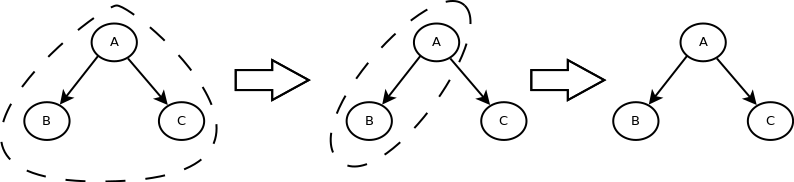
\includegraphics[width=\textwidth]{prototypes.png}

(The dashed region corresponds to which services that are embedded together)

This use-case is intended to show how we can easily go from a prototype where
we embed everything (this is easier to run locally) to hosting each service by
itself.

\begin{minted}{java}
// A.ol

ext outputPort A {
    Interfaces: AIface
}

ext outputPutPort B {
    Interfaces: BIface
}

constants {
    FOO: int
}
\end{minted}

\begin{minted}{java}
// A.col

include "B.col" // The includes work just like they do in Jolie
include "C.col"

// Previously called namespace. Configures makes it more explicit that we're
// talking about a specific package and not an arbitrary name
configures "A" {
    // Like always we just put the definitions here
    FOO = 42

    // We alter the syntax slightly for output ports being embedded
    outputPort B embeds B
    // The second B refers to the profile B (if no profile is specified it gets
    // the same name as the package it configures). This means that this
    // configures block also has name "A". It could also have been written as:
    // `profile "A" configures "A"`

    outputPort C embeds C
}
\end{minted}

Note: The previous proposal did not allow for embedding of services directly
from the configuration. This is however needed since packages by themselves
should be considered read-only. Thus if we want to configure a package to embed
its dependencies, then this must be done from external configuration, we cannot
do this in source.

\begin{minted}{java}
// B.col

configures "B" {
    inputPort B {
        Location: "local"
    }
}
\end{minted}

\begin{minted}{java}
// C.col

configures "C" {
    inputPort C {
        Location: "local"
    }
}
\end{minted}

In order to use an external B we need to update "A.col":

\begin{minted}{java}
// A.col
include "C.col"

configures "A" {
    outputPort B {
        Location: "socket://b.example.org:8000"
        Protocol: sodep
    }
    outputPort C embeds C
}
\end{minted}

In order to update the deployment file of B we simply need to update the
input port to no longer be local.

\begin{minted}{java}
// B.col
configures "B" {
    inputPort B {
        Location: "socket://localhost:8000"
        Protocol: sodep
    }
}
\end{minted}

In most cases however this would be unnecessary since the default
configuration file for "B" could already include a default input port.

In that case we could simply deploy directly from the default configuration.
The restriction on configuration units to only configure a single package helps
a lot. This restriction means that we cannot from any node configure any other
node which isn't a direct child of it. Without this we wouldn't be able to
easily swap out one configuration unit for another.

\subsection{Changes to the Interpreter's Pipeline}




\chapter{Package Manager}
% Status: Draft

\section{Packages}

A Jolie Package is an extension of a Jolie Module. Recall that a Jolie Module
was defined as a collection of resources, a name, and optionally an entry-point
for the module. A package extends this concept by adding information required
for package management. % TODO Last sentence sucks

A Jolie Package is described by a package manifest. The package manifest is a JSON file, which is always placed at the root of the package, and must be
called \verb!package.json!. The fixed location allows for the package manager
to easily identify a package. The JSON format was chosen as it plain-text, and
easy to both read and write for both humans and machines.

In listing \ref{lst:simple_manifest} we show a simple package manifest. This
manifest showcases the most important features of the manifest.A complete
specification of the package manifest format can be seen in Appendix A. The
service that this manifest describes is shown in figure \ref{fig:simple_calc}.

\begin{listing}[H]
\begin{minted}{json}
{
    "name": "calculator",
    "main": "calc.ol",
    "description": "A simple calculator service",
    "authors": ["Dan Sebastian Thrane <dathr12@student.sdu.dk>"],
    "license" "MIT",
    "interfaceDependencies": [
        { "name": "math", "version": "1.0.0" }
    ],
    "dependencies": [
        { "name": "sum", "version": "1.2.X" },
        { "name": "multiplication", "version": "2.1.0" }
    ]
}
\end{minted}
\caption{A Simple Package Manifest}
\label{lst:simple_manifest}
\end{listing}

\begin{listing}[H]
\begin{minted}[linenos=false]{text}
                +--------------+     +-------+
                |              | ==> |  sum  |
                |              |     +-------+
                |  calculator  |
                |              |     +------------------+
                |              | ==> |  multiplication  |
                +--------------+     +------------------+
\end{minted}
\caption{A Calculator Service}
\label{fig:simple_calc}
\end{listing}

Lines 2-3 take care of the module definition. The remaining attributes,
however, are entirely unique to packages. Some attributes included in the
manifest are there for indexing and discoverability purposes, examples of such
attributes are shown in lines 4-6. The rest of the document describes the
dependencies of this package.

A JPM dependency is defined as a ``code dependency''. What this means is that
the dependencies listed, should only be packages that we depend on for code.
This might be different from the typical definition in microservices. For
example, one might state that the calculator also has a dependency on the
client who speaks to it. In JPM however, we will not need to list the client,
as we do not depend on any code that the client has (in fact we know nothing
about how the client works).

JPM deals with two different types of dependencies: interface dependencies, and
ordinary dependencies. These two serve similar, but slightly different
purposes, and all depends on how the dependency is to be used.

An ordinary dependency should be used if we wish to use the code of some other
service, and want to option of embedding it. This will tell JPM to download
both ordinary dependencies, as well as interface dependencies.

Interface dependencies are instead dependencies that are only required to
interface with the package itself, and dependencies we need to interface with
others. An interface dependency will only cause us to download the interface
dependencies of each sub-dependency.

% TODO Need an example and algorithm for this stuff!

The interface dependency type isn't common in other package managers, but
having multiple types of dependencies is fairy common.  For example, a package
manager might provide dependencies which are only used during testing, we see
this in Maven, or it might provide dependencies only used during development,
seen in NPM.


% Status: Draft

\section{Architecture}

% At this point we have covered the responsibilities of JPM. Here we will be
% discussing the actual technical details of JPM. As well as taking a deeper
% look into features provided, and why they are useful.

The entirety of the ecosystem around JPM is written in Jolie, using the
features that the Jolie Module System provides, along with the features that
JPM itself provides.

At the ten-thousand foot view of the architecture, it consists of three
core services, as shown in figure \ref{fig:high_level_arch}:

\begin{enumerate}

\item \textbf{Registry}: Responsible for serving packages known to the
registry.

\item \textbf{JPM}: Provides the back-end of JPM. This includes communication
with one, or more, registries, for example to download packages.

\item \textbf{CLI}: Provides the front-end of JPM. The front-end is responsible
for displaying a user-facing interface, and will communicate with the back-end
to perform the actual work.

\end{enumerate}

% TODO Replace with non-ascii
\begin{listing}[H]
\begin{minted}{text}
                +-----------+     +-------+     +------------+
                |  jpm-cli  | ==> |  jpm  | ==> |  registry  |
                +-----------+     +-------+     +------------+
\end{minted}
\caption{Ten-thousand foot view of the JPM architecture}
\label{fig:high_level_arch}
\end{listing}


% Status: Draft

\section{Registry}
\label{sec:registry}

Stuff we need to cover in this section:

\begin{itemize}
\item Core responsibilities, such as: publish and download
\item Secondary responsibilities: Package information and dependencies
\item Tertiary responsibilities: Users and groups
\item Once responsibilities are in place we should talk about how we split up
the work-load.
\end{itemize}

\section{Security}
\label{sec:security}

The authorization of JPM is implemented in the \security service. The \security
service provides two different services, which work together to form the
\security service:

\begin{enumerate}

    \item \textbf{An authentication system:} Responsible for proving identity
        of users.

    \item \textbf{An authorization system:} Responsible for deciding which
        users are allowed to do what.

\end{enumerate}

In this section, the client represents a service which uses the \security
services. The system is written to assume that a client \emph{is not} an actual
user. As a result most operations have been written to support various options
which should not be available to actual users. This means that when the
\security service is deployed, care must be taken to ensure that it is not
reachable by any ordinary user. Only the services which use the \security
service should be able to reach it. The services that use the \security
service, will then proxy only the relevant parts along.

\subsection{Authentication}
\label{sec:authentication}

The authentication system has a user based system. Users authenticate
themselves using a password. A group is a collection of users, which have an
associated set of permission. A single user may be part of many groups, it is
from groups that a user gains permission to use parts of the system. We cover
group permissions in Section \ref{sec:authorization}.

The authentication system is build following recommendations from
OWASP\autocite{OWASP1,OWASP2,OWASP3}. In this section the
authentication implementation, and rules surrounding the system are summarized.

\subsubsection*{Username and Password Rules}

The usernames used for the system are unique and case in-sensitive. The
username is required to be between 1 and 64 characters long. All character
types are allowed in usernames. Encoding of the usernames (and passwords) are
deployment dependent, specifically it depends on the protocol and its
configuration.

Passwords are case sensitive. The only limitation put on password is a length
requirement between 5 and 128 characters.

The maximum lengths used for these are mostly to establish reasonable limits.
Accepting an unlimited amount of data can be of concern for both storage and
amount of network traffic. For data that should be presented, i.e. username,
having a maximum is helpful for the design of user interfaces.

\subsubsection*{Storage}

The usernames and passwords are stored in a SQL database. The database itself,
along with its driver is configurable via the configuration system (See
Section \ref{sec:col}). Passwords are hashed with
BCrypt\footnote{BCrypt is a password hashing algorithm which has been used
by OpenBSD and others}\cite{provos1999future}, each individual password has
its own salt. ``Salting'' a password is the act of adding a randomly
generated string to each password. The salt itself isn't secret,
but is instead used to avoid precomputed reverse lookup tables for
the hashes (rainbow tables).

\subsubsection*{Security Concerns}

Limiting number of login attempts within a period is often recommended. This is
done to avoid brute-force attacks. This isn't possible in Jolie, since the
sender isn't available to Jolie user code. This is most likely due to the fact
that no unique sender ID exists, since Jolie can accept messages from various
types of networks.

\subsubsection*{Authentication Process}

We start the discussion of how the authentication process works by looking at
how a client will successfully authenticate itself, this is shown in Figure
\ref{fig:auth_process}.

During the initial request nothing special really happens. The \security
service collaborates with both the \bcrypt service, along with its own
database. The database contains both \txtl{user} objects and \txtl{session}
objects. The \txtl{user} object has already been explained, and simply contains
the username, the hash of the salted password, and the salt itself. The
\txtl{session} object represents an active session. It contains the actual
token, which is a string generated by a cryptographically secure random number
generator. Along with this token, the object contains a timestamp for
generation, and a reference to the user object which created the session. The
timestamp will be used for implementing timeouts for the session.

At the end of the initial request, the client receives the token. This token is
what the client will have to provide for every privileged operation.  An
invalidation of a session may occur. This would ordinarily happen due to a
logout, or potentially a timeout which is handled by the client. The \security
service also supports checking the ``freshness'' of a session token, by making
sure it isn't older than some amount of time. This could be useful for ensuring
re-authentication before critical operations, such as changing your password.

\begin{figure}
    \begin{center}
    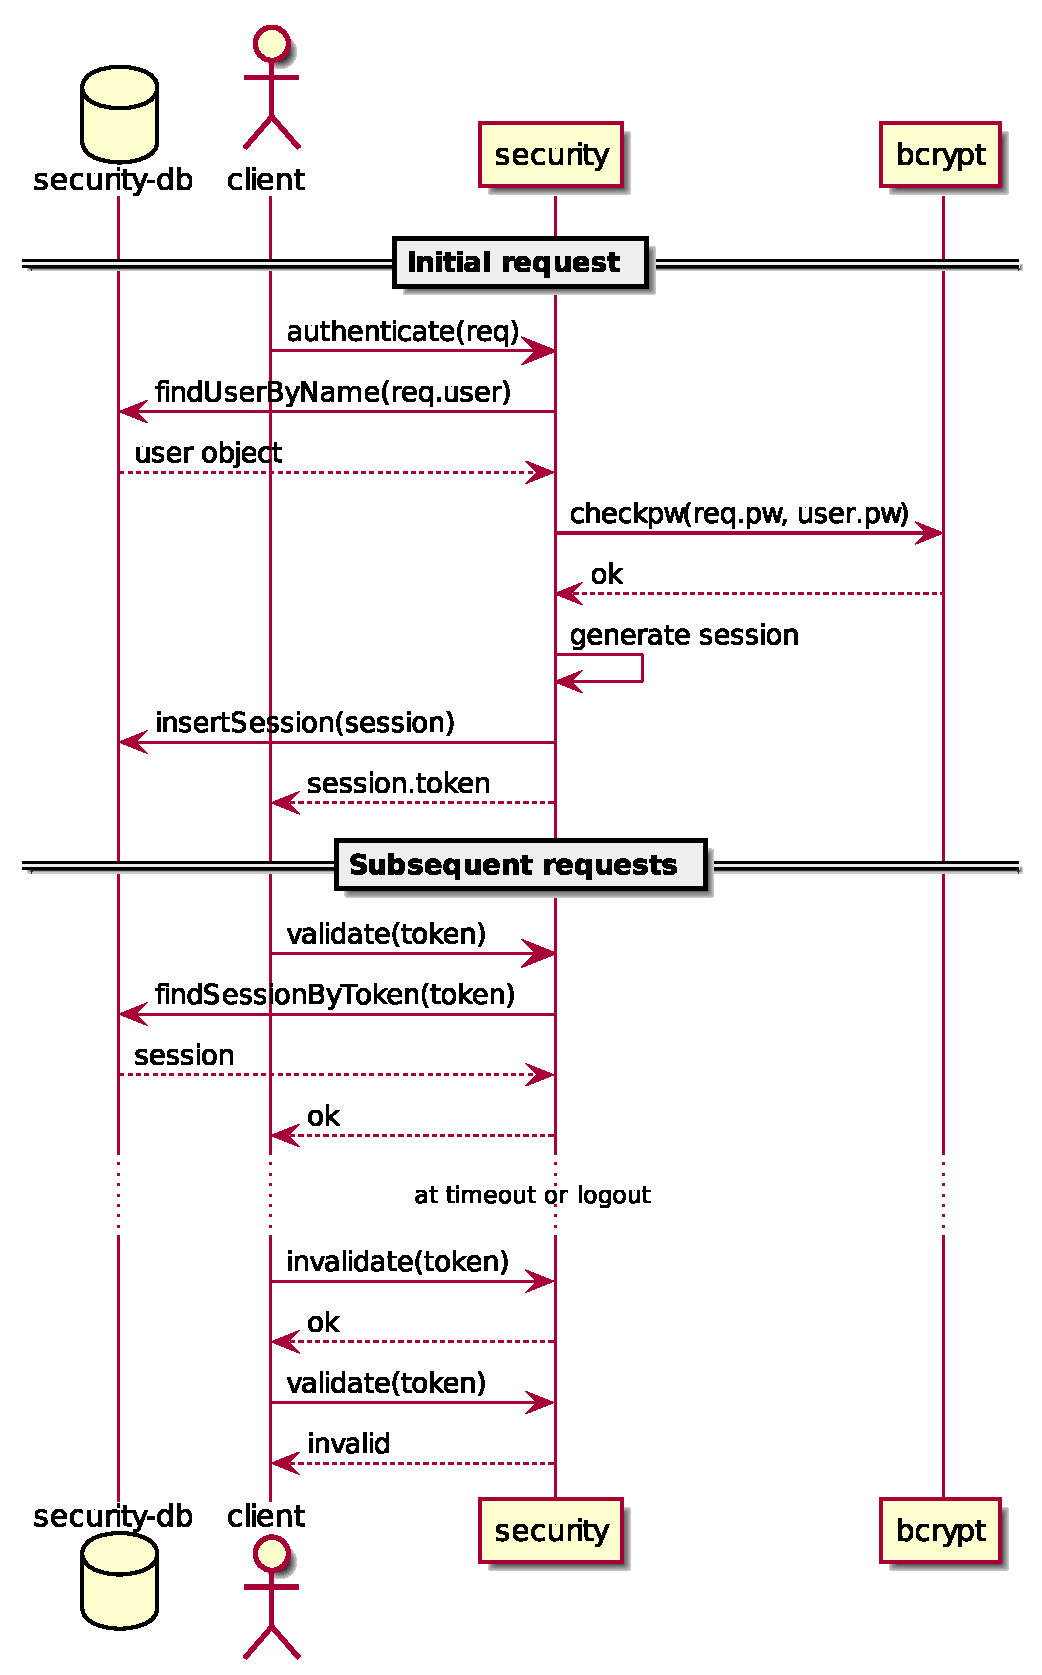
\includegraphics[width=0.8\textwidth]{package_manager/auth_sequence.eps}
    \end{center}
    \caption{The authentication process when successful}
    \label{fig:auth_process}
\end{figure}

Figure \ref{fig:auth_process} showed us the successful case. Internally,
validation will be performed at most steps. In the case of failure at
any of these steps a generic error message will be returned to the
client. The error message will only indicate if it was a user error or a
server error. This way an attacker cannot abuse the error messages for
information. For example given the error message ``Invalid password'' an
attacker would most likely be able to assume that the username itself is
correct.

\subsection{Authorization}
\label{sec:authorization}

The authorization system is based on an ``Access Control
Matrix''\cite{sandhu1994access} to define its security model. An access control
matrix, is a matrix $A$, where $A_{ij}$ contains the \emph{rights} that
\emph{role} $i$ has for \emph{resource} $j$.

A \emph{right} is a single piece of information. It describes something that an
entity is allowed to do for a specific resource in a role. In this
implementation a right is a simple string.

A \emph{resource} represents any entity that can have any rights associated
with it. This could, for example, be a file, which might have associated rights
such as ``read'' and ``write''.

A \emph{role} is some entity which have a set of rights for resources. In the
implementation roles are represented by \emph{groups}. A group is a
collection of users, which are provided by the authentication system.

Table \ref{tab:acm_example} shows an access control matrix for a few files,
which can be either read from or written to.

\begin{table}[H]
  \begin{center}
  \begin{tabular}{ | l | l | l | l | }
    \hline
            & \textbf{File 1}        & \textbf{File 2}      & \textbf{File 3}
    \\ \hline
    \textbf{Group 1} & read, write   & read                 &
    \\ \hline
    \textbf{Group 2} & read          & read                 & read, write
    \\ \hline
  \end{tabular}
  \end{center}

  \caption{A sample access control matrix for some computer files, which can be
      read from and written to by different groups}

  \label{tab:acm_example}
\end{table}

\subsection{Permissions in Registries}

The \registry service is the only consumer of the \security service. On top of
this service the \registry service implements the security model JPM uses. JPM
supports users these map one-to-one with the user model of the \security
service. On top of this JPM supports teams which are supported by a single
underlying group. The purpose of a team is to allow for multiple users to all
have ownership of a single package. Every single user and team get their own
group, user groups only have a single member, while a team group has members
corresponding to the team. The user groups are named \txtl{users.<name>}, and
teams \txtl{groups.<name>}.

When a package is downloaded from or published to the \registry the user's
permissions will be checked. For a user to download a package, the user must be
in a group having the \txtl{read} (or \txtl{write} for publishing) right for
the corresponding resource. Each package has an associated resource called
\txtl{packages.<name>}. A wild card resource (\txtl{packages.*}) also exists.
The wild card resource represents every single package, thus if a group holds
the \txtl{packages.*/read} right then that group is allowed to download ever
package in the \registry. This is exactly how a \registry might provide guest
downloads.

\subsection{Authentication in JPM}

When a user successfully authenticates, the authorization framework will
provide an authentication token proving the user's identity.

For user convenience the JPM system does not require a valid username and
password combination for every privileged operation. To avoid this, JPM will
store the authentication token returned by the \registry. These are stored in a
file on the file-system.

The authentication token is saved instead of the username and password.  Since
if an attacker were to gain access to both the username and password, she would
be able to gain full control over the user, this includes being able to
generate new authentication tokens.

If an attacker instead were to gain only the authentication token, the damage
is not as bad. The attacker would still be able to pose as the user, but only
while the authentication token is valid.

\section{The Command Line Interface}
\label{sec:cli}

The command line application serves as the user interface to JPM. The
application is, perhaps not unsurprisingly, named \mintinline{text}{jpm}. The
tool will be used in several examples.

The command line application is responsible for displaying a more user friendly
interface to inner workings of JPM. The tool will perform almost no work by
itself, but will instead delegate this to the back end (See Section TODO).

When first running the tool, the user will be welcomed with the following
message:

\begin{minted}{text}
JPM - The Jolie Package Manager
Version 1.0.0

Usage: jpm <COMMAND> <COMMAND-ARGUMENTS>

Command specific help: jpm help <COMMAND>

Available commands:
-------------------
init           Initializes a repository
search         Searches repositories for a package
install        Install dependencies
publish        Publish this package
start          Start this package.

[ Remaining commands removed from snippet ]
\end{minted}

As clearly visible form this snippet, for the tool to do any work we must first
give it something to do via a command. The commands that JPM understands almost
directly mirror the functionality provided by the back end. To use JPM to
create a new package, the user must simply use the \mintinline{text}{init}
command. This will display a prompt, guiding the user through the mandatory
field, and automatically create a package with the required structure. This
is shown in Listing \ref{lst:jpm_init}.

\begin{listing}[H]
\begin{minted}{text}
$ jpm init
Package name
------------
> my-package

Package description
-------------------
> This is my package

Author: [Format: name <email> (homepage)]
-----------------------------------------
> Dan Sebastian Thrane <dathr12@student.sdu.dk> (github.com/DanThrane)

Private package? [Y/n]
----------------------
> n

$ cat my-package/package.json | json name
my-package
\end{minted}

\caption{The \mintinline{text}{jpm} tool provides a user interface for common
    tasks. In this example, creating a new package.}

\label{lst:jpm_init}

\end{listing}

\subsection{Internal Organization and Deployment}

The command line tool delegates most of the work to the back end service.
Figure \ref{fig:cli_arch} shows the architecture from the CLI's point of view.

Most notably is the callback server, this server is responsible for receiving
information about events that occur in the back end. These are primarily used
to communicate progress, this is especially useful for long running processes,
   such as downloading dependencies. The back end will in these cases these
   events to a callback server, which can then choose to display information
   about this event. The need for a separate service comes mostly from a
   limitation in Jolie. In Jolie all communication follows either a one-way, or
   request-response communication pattern. As a result of this, it isn't
   possible for JPM to send back information while a request is being
   processed. To handle this the front end (in this case
           \mintinline{text}{jpm-cli}) will inform the back end of where it
   should send events.

\begin{listing}[H]
\begin{minted}{text}
                 +-------------------------------------+
                 | terminal (user)                     |
                 +-------------------------------------+
                                   |
                                   v
                 +-------------------------------------+
+------------+   |            embeds                   |
| console-ui |<--| jpm-cli ----------------+           |
+------------+   |                         |           |
+------------+   |                         v           |
| arg-parser |<--|                   +----------------+|
+------------+   |                   | callback       ||
                 |                   +----------------+|
                 +--------------------------^----------+
                                   |        |
                                   |        |
                                   v        |
                 +-------------------------------------+
                 |           jpm (back-end)            |
                 +-------------------------------------+
                     |         |         |         |
                     v         v         v         v
                 +-------+ +-------+ +-------+ +-------+
                 | reg-a | | reg-b | | reg-c | | reg-d |
                 +-------+ +-------+ +-------+ +-------+
\end{minted}
\caption{The system architecture from the CLI's point of view}
\label{fig:cli_arch}
\end{listing}

Quite a lot of services exists on the client side, notably
\mintinline{text}{jpm-cli} and \mintinline{text}{jpm}. From a usability
perspective this is less optimal. For this reason the \mintinline{text}{jpm}
binary, which ships with the package manager, will use a deployment which
embeds all of the core services together. Future versions of the package
manager, may wish to optionally spin up the required services, and run them as
daemons\footnote{A daemon is a background process running on a computer}. This
will remove quite a bit of the overhead associated with spinning up the JVM
(required for the Jolie engine) and every embedded service. Such a practice is
done by similar tools, as an example the JVM based build tool Gradle provides
such a daemon\autocite{GRAA}.  This conversion would be relatively straight
forward, since the server architecture required by the daemon is already
implemented.

% Status: draft

\section{Integrity Checks}

This is a section about integrity checks in JPM.

\begin{itemize}
    \item Some background about checksums (probably)
    \item How we do it. Reason we don't go for something like code signing
        (in pkg manager)
    \item Code signing, and why we would prefer this.
\end{itemize}



\appendix
\chapter{Appendix}
\section{Appendix A: JPM Manifest Specification}\label{package-specification}

This document covers the specification of the file which defines a
package. The format used for this document will be JSON, but the format
and whether or not to allow for several documents is still up for
discussion. For now we should avoid using any features which the generic
Jolie value cannot support.

\subsection{Purpose}\label{purpose}

The purpose of the package document is to define what a package is.
Every Jolie package will contain such a document, and it describes
several important properties about the package. These properties are
described in the section ``Format and Properties''.

\subsection{Table of Contents}\label{table-of-contents}

\begin{itemize}
\tightlist
\item
  \protect\hyperlink{format-and-properties}{Format and Properties}

  \begin{itemize}
  \tightlist
  \item
    \protect\hyperlink{name}{name}
  \item
    \protect\hyperlink{version}{version}
  \item
    \protect\hyperlink{license}{license}
  \item
    \protect\hyperlink{authors}{authors}
  \item
    \protect\hyperlink{private}{private}
  \item
    \protect\hyperlink{main}{main}
  \item
    \protect\hyperlink{dependencies}{dependencies}
  \item
    \protect\hyperlink{dependency}{dependency}

    \begin{itemize}
    \tightlist
    \item
      \protect\hyperlink{name-1}{name}
    \item
      \protect\hyperlink{version-1}{version}
    \item
      \protect\hyperlink{registry}{registry}
    \end{itemize}
  \item
    \protect\hyperlink{registries}{registries}
  \item
    \protect\hyperlink{registry-1}{registry}

    \begin{itemize}
    \tightlist
    \item
      \protect\hyperlink{name-2}{name}
    \item
      \protect\hyperlink{location}{location}
    \end{itemize}
  \end{itemize}
\end{itemize}

\hypertarget{format-and-properties}{\subsection{Format and
Properties}\label{format-and-properties}}

\hypertarget{name}{\subsubsection{name}\label{name}}

\textbf{Name:} \texttt{name}

\textbf{Optional:} false

\textbf{Type:} \texttt{string}

\textbf{Description:} The \texttt{name} property uniquely defines a
package in a registry. Every registry must only contain a single package
with a given name.

\textbf{Rules:}

\begin{itemize}
\tightlist
\item
  The name of a package is \emph{not} case-sensitive
\item
  The length of a name is less than 255 characters
\item
  Names are US-ASCII
\item
  Names may only contain unreserved URI characters (see section 2.3 of
  \href{https://www.ietf.org/rfc/rfc3986.txt}{RFC 3986})
\end{itemize}

If any of these rules are broken the JPM tool should complain when
\emph{any} command is invoked. Similarly a registry should reject any
such package.

\hypertarget{version}{\subsubsection{version}\label{version}}

\textbf{Name:} \texttt{version}

\textbf{Optional:} false

\textbf{Type:} \texttt{string}

\textbf{Description:} This property describes the current version of
this package.

\textbf{Rules:}

\begin{itemize}
\tightlist
\item
  The version string must be a valid SemVer 2.0.0 string (see
  http://semver.org/spec/v2.0.0.html)
\end{itemize}

\hypertarget{license}{\subsubsection{license}\label{license}}

\textbf{Name:} \texttt{property\_name}

\textbf{Optional:} false

\textbf{Type:} \texttt{string}

\textbf{Description:} Describes the license that this package is under.

\textbf{Rules:}

\begin{itemize}
\tightlist
\item
  Must be a valid identifier. See https://spdx.org/licenses/
\end{itemize}

\hypertarget{authors}{\subsubsection{authors}\label{authors}}

\textbf{Name:} \texttt{authors}

\textbf{Optional:} false

\textbf{Type:}
\texttt{string\textbar{}array\textless{}string\textgreater{}}

\textbf{Description:} Describes the authors of this package

\textbf{Rules:}

\begin{itemize}
\tightlist
\item
  The array must contain at least a single entry
\item
  Each entry should follow this grammar:
\end{itemize}

\begin{verbatim}
name ["<" email ">"] ["(" homepage ")"]
\end{verbatim}

\hypertarget{private}{\subsubsection{private}\label{private}}

\textbf{Name:} \texttt{private}

\textbf{Optional:} true

\textbf{Type:} \texttt{boolean}

\textbf{Description:} Describes if this package should be considered
private. If a package is private it cannot be published to the
``public'' repository.

\textbf{Rules:}

\begin{itemize}
\tightlist
\item
  By default this property has the value of \texttt{true} to avoid
  accidential publishing of private packages.
\end{itemize}

\hypertarget{main}{\subsubsection{main}\label{main}}

\textbf{Name:} \texttt{main}

\textbf{Optional:} true

\textbf{Type:} \texttt{string}

\textbf{Description:} Describes the main file of a package.

\textbf{Rules:}

\begin{itemize}
\tightlist
\item
  The value is considered to be a relative file path from the package
  root.
\end{itemize}

\hypertarget{dependencies}{\subsubsection{dependencies}\label{dependencies}}

\textbf{Name:} \texttt{dependencies}

\textbf{Optional:} true

\textbf{Type:} \texttt{array\textless{}dependency\textgreater{}}

\textbf{Description:} Contains an array of dependencies. See the
``dependency'' sub-section for more details.

\textbf{Rules:}

\begin{itemize}
\tightlist
\item
  If the property is not listed, a default value of an empty array
  should be used
\end{itemize}

\hypertarget{dependency}{\subsubsection{dependency}\label{dependency}}

\textbf{Type:} \texttt{object}

\textbf{Description:} A dependency describes a single dependency of a
package. This points to a package at a specific point on a specific
registry.

\hypertarget{name-1}{\paragraph{name}\label{name-1}}

\textbf{Name:} \texttt{name}

\textbf{Optional:} false

\textbf{Type:} \texttt{string}

\textbf{Description:} Describes the name of the dependency. This refers
to the package name, as defined earlier.

\textbf{Rules:} A dependency name follows the exact same rules as a
package name.

\hypertarget{version-1}{\paragraph{version}\label{version-1}}

\textbf{Name:} \texttt{version}

\textbf{Optional:} false

\textbf{Type:} \texttt{string}

\textbf{Description:} Describes the version to use

\textbf{Rules:}

\begin{itemize}
\tightlist
\item
  Must be a valid SemVer 2.0.0 string
\item
  (This property follows the same rules as the package version does)
\end{itemize}

\hypertarget{registry}{\paragraph{registry}\label{registry}}

\textbf{Name:} \texttt{registry}

\textbf{Optional:} true

\textbf{Type:} \texttt{string}

\textbf{Description:} This describes the exact registry to use. If no
registry is listed the ``public'' registry will be used.

\textbf{Rules:}

\begin{itemize}
\tightlist
\item
  The value of this property must be a valid registry as listed in the
  \texttt{registries} property.
\end{itemize}

\hypertarget{registries}{\subsubsection{registries}\label{registries}}

\textbf{Name:} \texttt{registries}

\textbf{Optional:} true

\textbf{Type:} \texttt{array\textless{}registry\textgreater{}}

\textbf{Description:} Contains an array of known registries. See the
registry sub-section for more details.

\textbf{Rules:}

\begin{itemize}
\tightlist
\item
  This property contains an implicit entry which points to the public
  registry. This registry is named ``public''.
\end{itemize}

\hypertarget{registry-1}{\subsubsection{registry}\label{registry-1}}

\textbf{Type:} \texttt{object}

\textbf{Description:} A registry describes a single JPM registry. A JPM
registry is where the package manager can locate a package, and also
request a specific version of a package.

\hypertarget{name-2}{\paragraph{name}\label{name-2}}

\textbf{Name:} \texttt{name}

\textbf{Optional:} false

\textbf{Type:} \texttt{string}

\textbf{Description:} This property uniquely identifies the registry.

\textbf{Rules:}

\begin{itemize}
\tightlist
\item
  A name cannot be longer than 1024 characters
\item
  The name cannot be ``public''
\item
  No two registries may have the same name
\end{itemize}

\textbf{TODO:}

\begin{itemize}
\tightlist
\item
  Encoding of name
\item
  Should the length limit be dropped? There is no technical reason for
  the limit
\end{itemize}

\hypertarget{location}{\paragraph{location}\label{location}}

\textbf{Name:} \texttt{location}

\textbf{Optional:} false

\textbf{Type:} \texttt{string}

\textbf{Description:} Describes the location of the registry.

\textbf{Rules:}

\begin{itemize}
\tightlist
\item
  Must be a valid Jolie location string (e.g.
  ``socket://localhost:8080'')
\end{itemize}



\end{document}
